% Defines Figure~\ref{fig:pfs_coverage}, which contributions/future_new_programs.tex also references via \ref.
% If you drop this file, either keep future_new_programs.tex's figure reference intact by moving this
% wrapfigure elsewhere, or remove that reference so it doesn't render as "??".
\textbf{Astronomical Instruments to Maximize LSST data:}
In the \LSST\ era, the central bottleneck will not be imaging depth, but rather spectroscopic capacity.
% : both dark and bright siren measurements ultimately require secure redshifts of host galaxies and rapid characterization of transients from \LSST's alert stream. 
To aid in this effort, I will test and deploy advanced focal plane technology for future multi-object spectrographs.
As part of this focus, I will explore instrument design for a multi-object spectrograph optimized for standard siren cosmology, specialized for the precision and 
event rates of forthcoming gravitational wave detectors. 
This instrument would serve two goals: 1) characterize astrophysical transients associated with potential bright standard sirens, and 2) obtain spectroscopic redshifts from host galaxies to bolster dark siren measurements. Through this dual purpose, the proposed instrument would become a dark energy science machine primed to capitalize on the deluge of data from \LSST\ and future GW observatories. % MOS instrumentation development
These pathfinding activities would help to inform the proposed \specsfive, a future, large-scale cosmic frontier experiment \cite{2025arXiv250307923B}. Developing and testing of focal-plane technology will help shape the capabilities of \specsfive, so it serves as an effective spectroscopic complement to \Rubin\ starting in the mid-2030's. % Spec-S5 instrumentation development.
\begin{wrapfigure}{r}{0.5\textwidth} % 'r' for right, 'l' for left
    \centering
    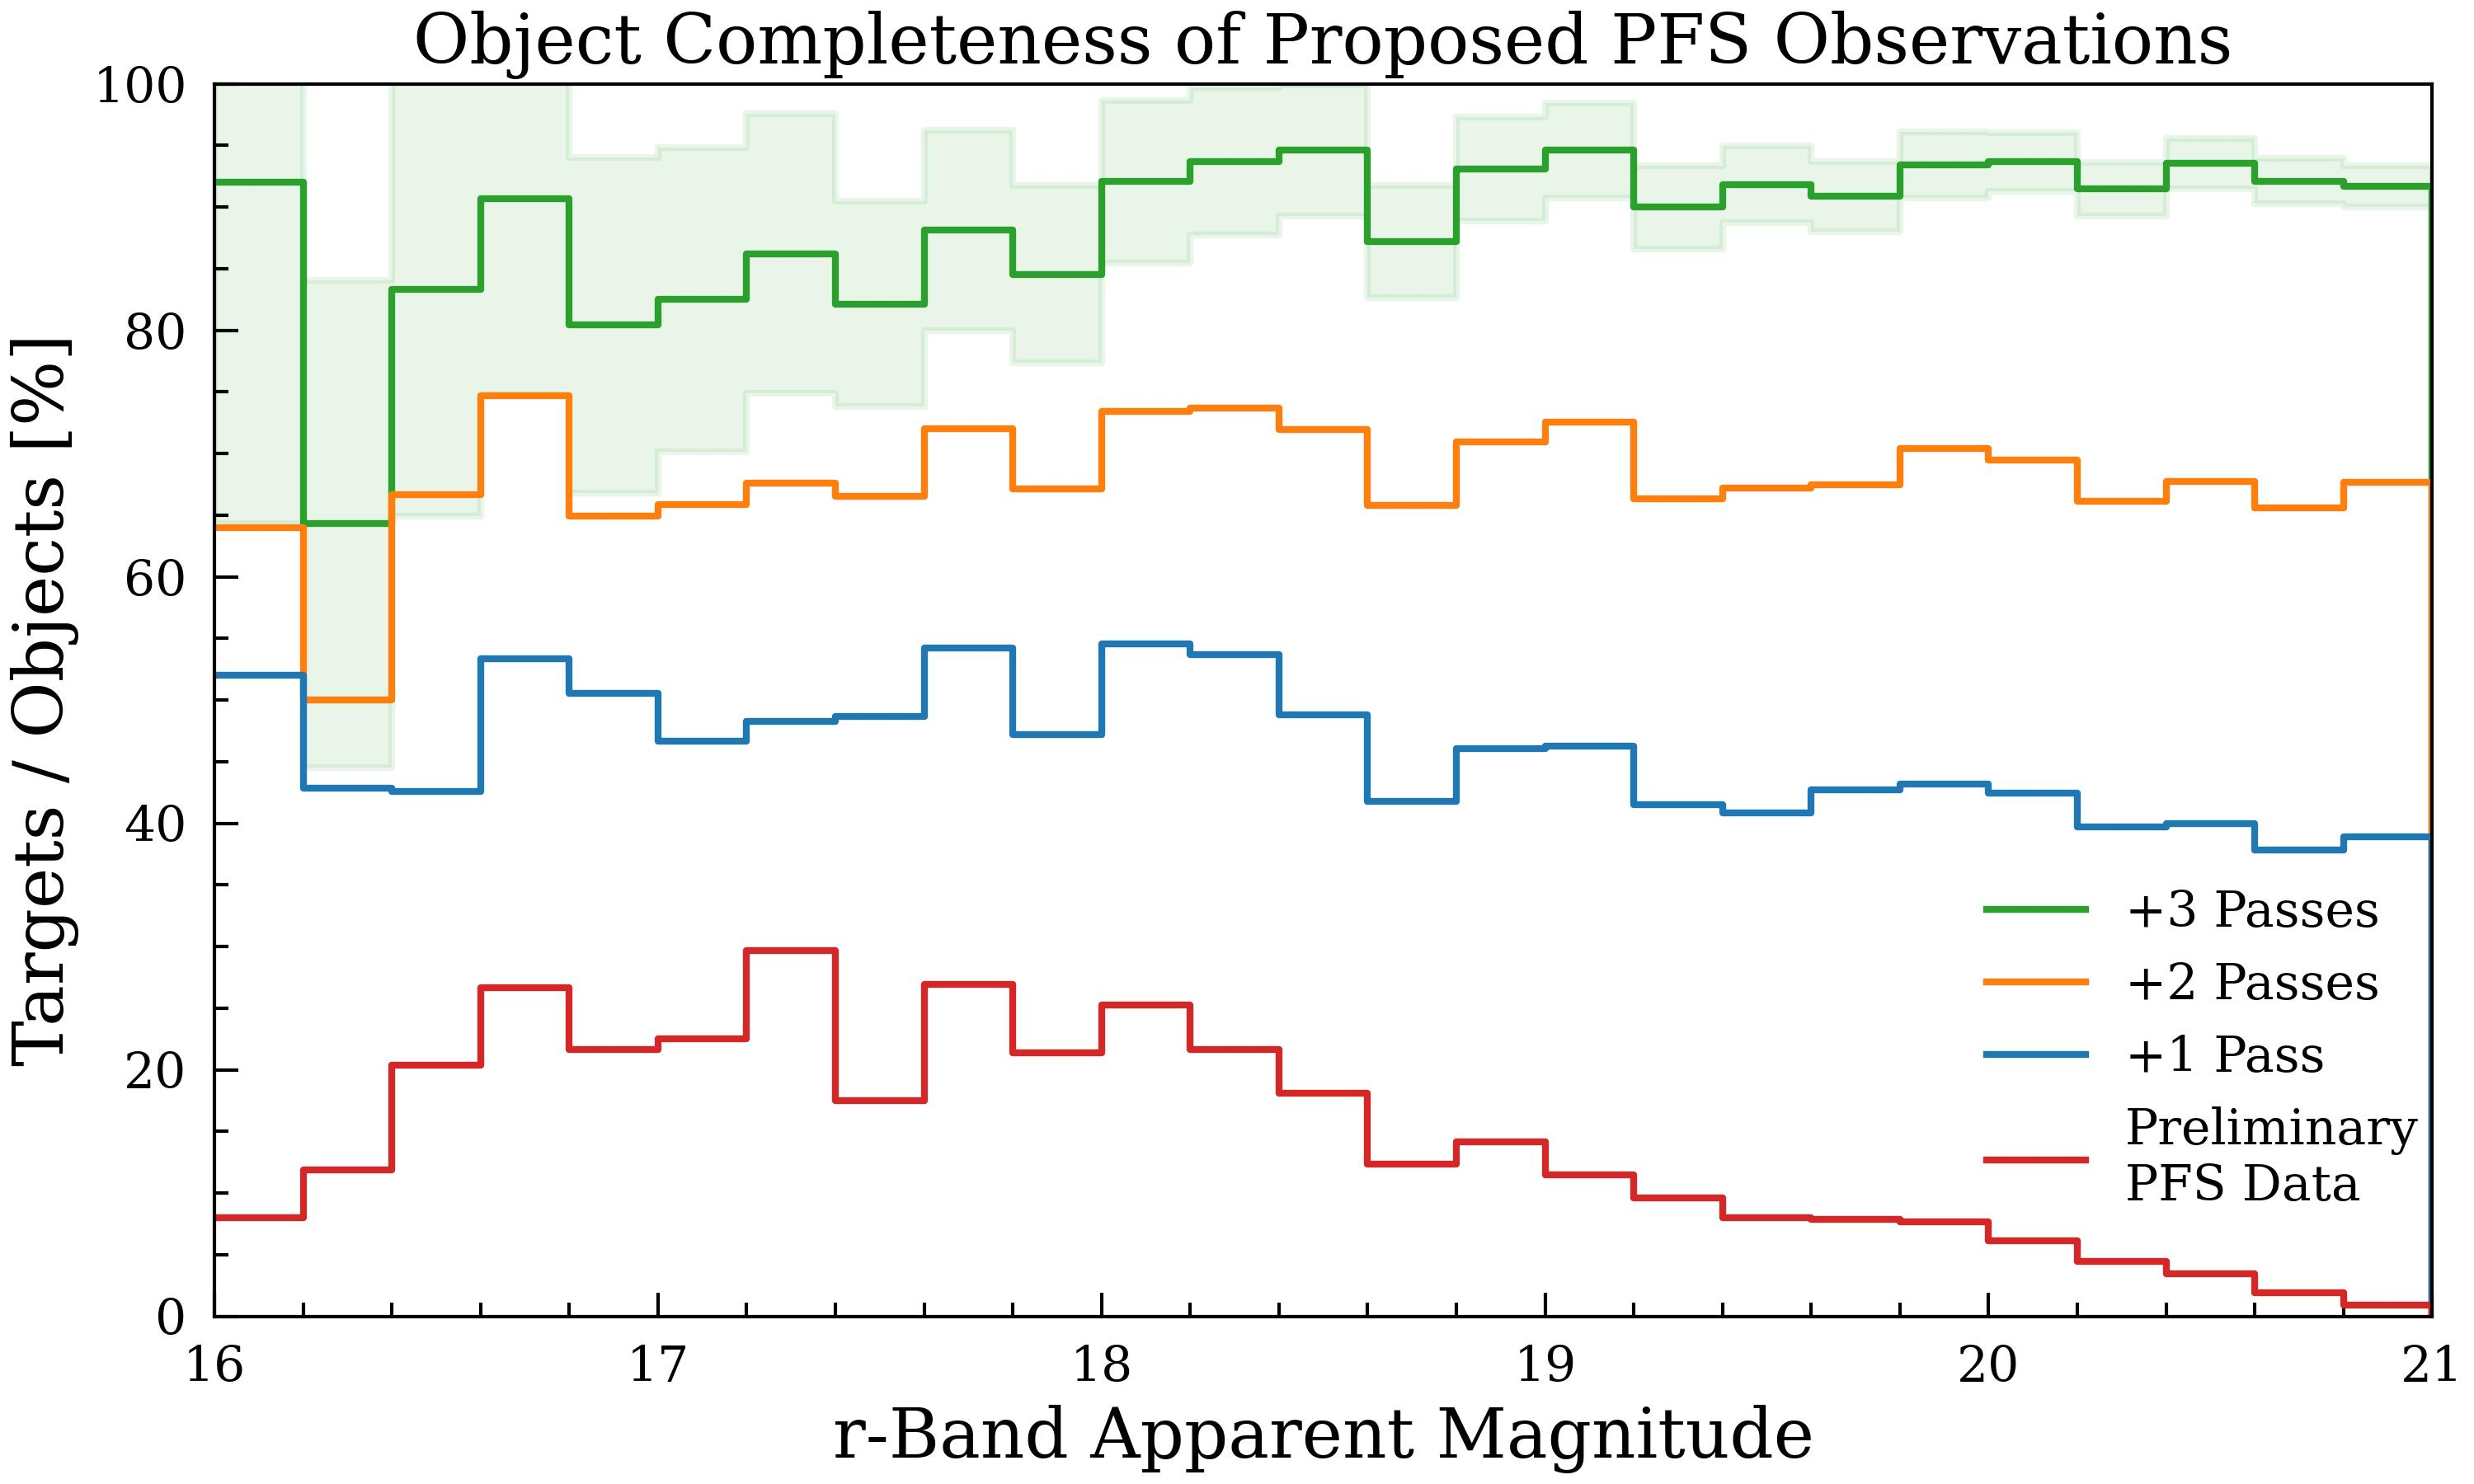
\includegraphics[width=0.5\textwidth]{figures/pfs_completeness.png}
	\caption{In red, the completeness of \PFS\ objects acquired as part of our \ToO\ campaign \cite{Zhang2025S250328ae}, with other colors showing the forecasted completeness of proposed observations. The high completeness obtained over the localization region in 3 passes (one night) demonstrates the utility of current and future multi-object spectrographs as characterization machines for standard siren cosmology.}
    \label{fig:pfs_coverage}
\end{wrapfigure}
I will continue in a support-scientist role for LSSTCam as the \LSST\ transitions into survey operations, maintaining the operational knowledge needed to respond quickly to sensor anomalies and focal-plane issues as they arise.
Building on my commissioning-era characterization of focal-plane defects, I will deploy a defect-monitoring tool, currently in-development, to \texttt{cp\_verify}, the calibration-product verification framework used by the \LSST\ Science Pipelines \cite{10.71929/rubin/2570545}. This tool will elevate defect monitoring to an automated process, directly improving the quality of \LSST\ data.